\documentclass[tikz,border=0pt]{standalone}
\begin{document}
% Cell 5 of the honeycomb strip, exactly as the paper writes it, drawn on the page so the PDF can be
% measured: the box's bottom edge is the floor the thick arc has to sit on, and the arc's own control
% points are read out of the PDF curve. border=0pt keeps the page flush with the drawing.
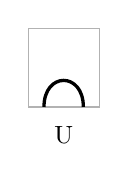
\begin{tikzpicture}[x=1cm,y=1cm,font=\small]
 \begin{scope}[xshift={1.45*mod(5,5)*1cm},yshift={-2.1*floor(5/5)*1cm}]
 \draw[black!30] (-.45,0) rectangle (.45,1);
 \draw[very thick] (-.25,0) .. controls (-.25,.45) and (.25,.45) .. (.25,0);
 \node at (0,-.35) {U};
 \end{scope}
\end{tikzpicture}
\end{document}
